\documentclass[11pt]{article}
\usepackage[margin=1in]{geometry}
\usepackage[T1]{fontenc}
\usepackage[utf8]{inputenc}
\usepackage{lmodern}
\usepackage{amsmath}
\usepackage{amssymb}
\usepackage{booktabs}
\usepackage{array}
\usepackage{hyperref}
\usepackage{pgfplots}
\usepackage{tikz}
\usepackage{enumitem}
\usepackage{setspace}
\pgfplotsset{compat=1.18}

\title{\textbf{Do Leaders Export Pollution While Importing Wealth?}\\[0.35em]
\large Midterm Report}
\author{Richard Schulz \and Ruby Wang \and Muhammad Majid Altaf}
\date{\today}

\begin{document}
\maketitle
\thispagestyle{empty}

\begin{abstract}
We study whether national leaders direct cleaner economic growth to their birth regions rather than simply more growth. Our empirical strategy combines PLAD birth-region information, harmonized nighttime lights, ACAG surface NO$_2$, V-Dem democracy scores, and GADM ADM2 boundaries in a global district-year panel with region and country-year fixed effects. The report delivers three main findings. First, we replicate the classic regional favoritism result in the long 1992--2013 nightlights sample. Second, that first stage weakens sharply in later windows: the birth-region coefficient remains positive through 2000--2013 but largely disappears in 2005--2013 and in the broader 2005--2019 harmonized window. Third, once attention shifts to the proposal-aligned pollution sample, we do not find evidence of ``green favoritism'': pooled NO$_2$ and pollution-intensity coefficients are weakly positive, and a parallel PM$_{2.5}$ extension reinforces the same conclusion. The central issue for the second half of the project is therefore not data construction but interpretation: the environmental extension is now feasible, but it rests on a first stage that attenuates substantially in the post-2005 period.
\end{abstract}

\section{Project Status and Research Question}
Our research question is whether leaders channel cleaner forms of economic development to their own birth regions while leaving dirtier activity to politically peripheral districts. The intended empirical signature is a positive treatment effect on nighttime lights combined with a zero or negative treatment effect on pollution. This question extends the classic regional-favoritism literature into environmental outcomes: if leaders steer economic activity toward their home districts, does that activity come with more or less pollution than would be expected given its scale?

The midterm milestone focused on assembling a proposal-aligned 2005--2019 panel using ACAG NO$_2$ data, harmonized nightlights, and PLAD treatment coding at ADM2 level. All three core datasets are now linked at ADM2 resolution, and a longer-window PM$_{2.5}$ extension has been added as a parallel robustness check. The main empirical challenge that has emerged is not data construction but the attenuation of the nightlights first stage in the post-2005 period, which constrains the interpretation of the pollution-side results.

\section{Annotated Bibliography}
\begin{enumerate}[leftmargin=*, itemsep=0.5em]
    \item \textbf{Hodler and Raschky (2014), ``Regional Favoritism.''} This is the foundational paper for the project. It shows that national leaders direct more economic activity, proxied by nightlights, to their birth regions; our design is a direct environmental extension of this logic.

    \item \textbf{Bora (2025), ``Birthplace Favoritism Revisited.''} Bora provides the most relevant modern replication benchmark for the lights specification. The paper reproduces the classic birthplace-favoritism result in an open-source framework, shows that it survives when the original Hodler--Raschky DMSP window is extended from 1992--2009 to 1992--2014, and then separately confirms persistence in the VIIRS era from 2012--2025. Notably, Bora analyzes DMSP and VIIRS eras separately and does not estimate a panel spanning both sensor systems, so the paper does not speak to how the first stage behaves under harmonization. This matters for us because it provides a current benchmark for how far the nightlights first stage can travel under alternative data choices and longer windows, while leaving open the question we face in our harmonized 2005--2019 panel.

    \item \textbf{Bomprezzi et al. (2025), PLAD.} PLAD provides leader birth-region identifiers at subnational level and makes a global ADM2 treatment design feasible. It is the core political dataset used to define treated birth districts and leader spells.

    \item \textbf{Cooper et al. (2022), global fine-scale ambient NO$_2$.} This paper underlies the ACAG NO$_2$ product we now use. It is important because it delivers annual fine-resolution surface NO$_2$ estimates that are much better suited to an ADM2 panel than coarser satellite-only products.

    \item \textbf{Elvidge et al. (2013), ``Why VIIRS data are superior to DMSP.''} This paper is the key reference for the nightlights side of the project. It explains the DMSP--VIIRS sensor transition and why harmonization matters for any panel that spans both systems.

    \item \textbf{Copeland and Taylor (2004), ``Trade, Growth, and the Environment.''} This is not a favoritism paper, but it provides the environmental-economics intuition behind our project. We adapt the pollution-haven logic from cross-border settings to within-country political geography.
\end{enumerate}

\section{Datasets and Descriptive Analysis}
This section sets up the comparison that runs through the rest of the report: a long nightlights replication sample, a later 2005--2019 joint NO$_2$ and nightlights sample, and a longer-window PM$_{2.5}$ extension. Table~\ref{tab:data-summary} summarizes the datasets behind those panels, while Table~\ref{tab:sample-support} summarizes sample composition and treatment support across the three analysis panels.

\begin{table}[h]
\centering
\caption{Dataset summary}
\label{tab:data-summary}
\small
\begin{tabular*}{\textwidth}{@{\extracolsep{\fill}}p{3.0cm}p{1.8cm}p{2.0cm}p{7.0cm}}
\toprule
Dataset & Coverage & Unit & Current use \\
\midrule
PLAD & 148 countries in analysis window & Leader-year / birth district & Birth-region treatment and leader spell construction \\
Nightlights & 2005--2019 & ADM2-year & Harmonized DMSP (2005--2013) and simVIIRS (2014--2019) \\
ACAG surface NO$_2$ & 2005--2019 & ADM2-year & Main pollution outcome in the proposal-aligned panel \\
ACAG SatPM PM$_{2.5}$ & 1998--2024 & ADM2-year & Parallel pollution extension; longer-window robustness check beyond the ACAG NO$_2$ sample \\
V-Dem polyarchy & 2005--2019 & Country-year & Democracy interaction and autocracy subsamples \\
GADM v4.1 & Static & ADM2 polygon & Common spatial aggregation unit \\
\bottomrule
\end{tabular*}
\end{table}

\begin{table}[h]
\centering
\caption{Sample composition and treatment support across analysis panels}
\label{tab:sample-support}
\small
\resizebox{\textwidth}{!}{%
\begin{tabular}{lrrrrrrr}
\toprule
Panel & Years & Obs & Regions & Countries & Treated obs & Treated share & Leader-period clusters \\
\midrule
Replication nightlights & 1992--2013 & 951{,}915 & 46{,}566 & 235 & 2{,}522 & 0.0026 & 2{,}723 \\
Joint NO$_2$ + nightlights & 2005--2019 & 673{,}137 & 47{,}463 & 230 & 1{,}590 & 0.0024 & 1{,}874 \\
PM$_{2.5}$ extension & 1998--2024 & 1{,}289{,}925 & 47{,}775 & 238 & 2{,}853 & 0.0022 & 3{,}855 \\
\bottomrule
\end{tabular}
}
\end{table}

For the descriptive figure below, we define pollution intensity as $\ln(\text{NO}_2+0.01)-\ln(\text{Nightlights}+0.01)$. Higher values therefore correspond to more pollution relative to observed economic activity. The raw comparison suggests that leader birth regions are brighter on average and also exhibit lower pollution intensity, consistent with being economically stronger and somewhat greener, but this pattern is purely descriptive rather than causal. It nevertheless helps motivate the fixed-effects results below by showing that the central puzzle is not whether leader regions look different in levels, but whether those differences survive once comparisons are made within region and country-year.

\begin{figure}[h]
\centering
\begin{minipage}{0.48\textwidth}
\centering
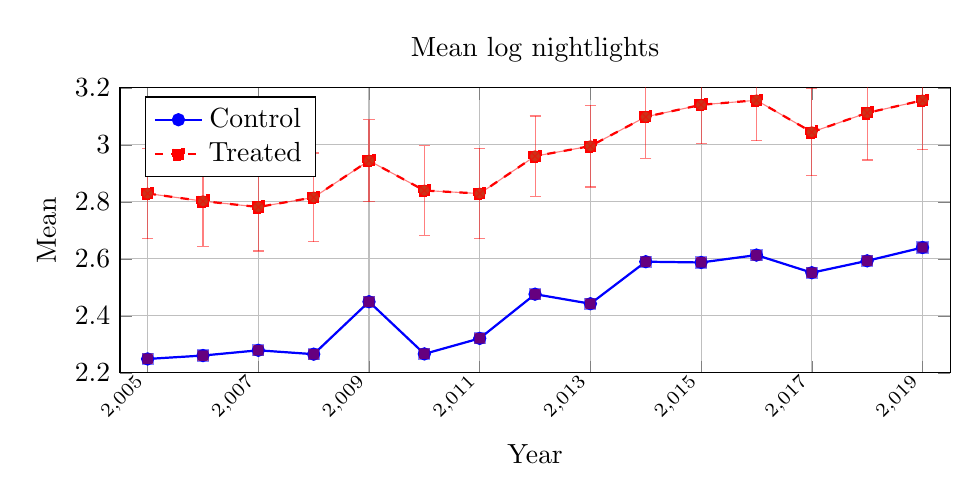
\begin{tikzpicture}
\begin{axis}[
    width=\textwidth,
    height=5.2cm,
    title={Mean log nightlights},
    xlabel={Year},
    ylabel={Mean},
    xmin=2004.5, xmax=2019.5,
    ymin=2.2, ymax=3.2,
    xtick={2005,2007,2009,2011,2013,2015,2017,2019},
    xticklabel style={rotate=45, anchor=east, font=\scriptsize},
    legend pos=north west,
    grid=major,
]
\addplot[blue, thick, mark=*] coordinates {
(2005,2.248639) (2006,2.260563) (2007,2.278933) (2008,2.265338) (2009,2.449487)
(2010,2.266320) (2011,2.320744) (2012,2.475901) (2013,2.442373) (2014,2.589918)
(2015,2.587222) (2016,2.613174) (2017,2.551299) (2018,2.592977) (2019,2.639725)};
\addplot+[blue, forget plot, opacity=0.5, error bars/.cd, y dir=both, y explicit]
coordinates {
(2005,2.248639) +- (0,0.006543)
(2006,2.260563) +- (0,0.006792)
(2007,2.278933) +- (0,0.006612)
(2008,2.265338) +- (0,0.006688)
(2009,2.449487) +- (0,0.006053)
(2010,2.266320) +- (0,0.006751)
(2011,2.320744) +- (0,0.006337)
(2012,2.475901) +- (0,0.005934)
(2013,2.442373) +- (0,0.005960)
(2014,2.589918) +- (0,0.005723)
(2015,2.587222) +- (0,0.005694)
(2016,2.613174) +- (0,0.005794)
(2017,2.551299) +- (0,0.005605)
(2018,2.592977) +- (0,0.005612)
(2019,2.639725) +- (0,0.005693)};
\addlegendentry{Control}
\addplot[red, thick, dashed, mark=square*] coordinates {
(2005,2.829280) (2006,2.802476) (2007,2.781867) (2008,2.815536) (2009,2.944598)
(2010,2.839817) (2011,2.829081) (2012,2.960400) (2013,2.995746) (2014,3.098433)
(2015,3.140525) (2016,3.156481) (2017,3.044752) (2018,3.112202) (2019,3.156147)};
\addplot+[red, forget plot, opacity=0.5, error bars/.cd, y dir=both, y explicit]
coordinates {
(2005,2.829280) +- (0,0.159356)
(2006,2.802476) +- (0,0.158343)
(2007,2.781867) +- (0,0.154222)
(2008,2.815536) +- (0,0.155873)
(2009,2.944598) +- (0,0.144056)
(2010,2.839817) +- (0,0.156948)
(2011,2.829081) +- (0,0.158243)
(2012,2.960400) +- (0,0.141076)
(2013,2.995746) +- (0,0.143596)
(2014,3.098433) +- (0,0.145512)
(2015,3.140525) +- (0,0.136609)
(2016,3.156481) +- (0,0.142380)
(2017,3.044752) +- (0,0.153639)
(2018,3.112202) +- (0,0.165419)
(2019,3.156147) +- (0,0.173688)};
\addlegendentry{Treated}
\end{axis}
\end{tikzpicture}
\end{minipage}
\hfill
\begin{minipage}{0.48\textwidth}
\centering
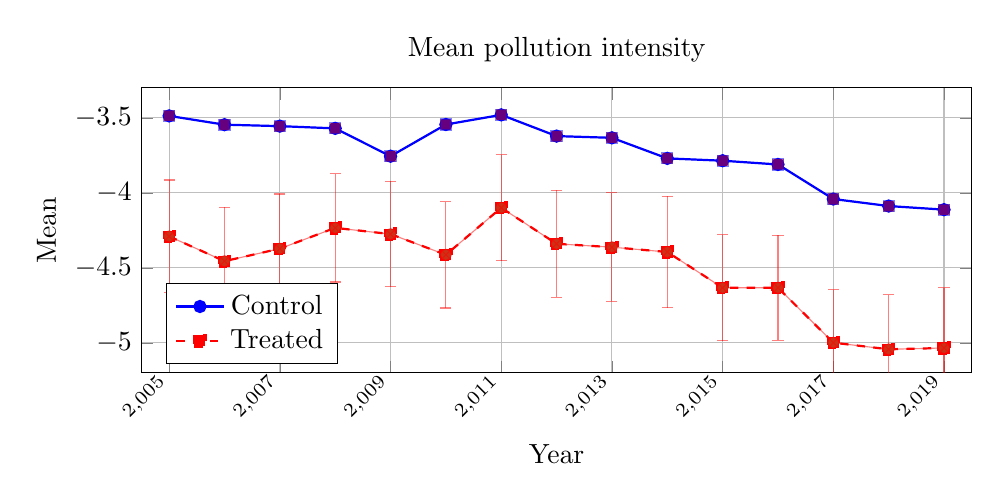
\begin{tikzpicture}
\begin{axis}[
    width=\textwidth,
    height=5.2cm,
    title={Mean pollution intensity},
    xlabel={Year},
    ylabel={Mean},
    xmin=2004.5, xmax=2019.5,
    ymin=-5.2, ymax=-3.3,
    xtick={2005,2007,2009,2011,2013,2015,2017,2019},
    xticklabel style={rotate=45, anchor=east, font=\scriptsize},
    legend pos=south west,
    grid=major,
]
\addplot[blue, thick, mark=*] coordinates {
(2005,-3.486899) (2006,-3.545470) (2007,-3.555166) (2008,-3.570129) (2009,-3.755735)
(2010,-3.544344) (2011,-3.479974) (2012,-3.621586) (2013,-3.633062) (2014,-3.770262)
(2015,-3.785750) (2016,-3.810862) (2017,-4.041157) (2018,-4.088054) (2019,-4.112027)};
\addplot+[blue, forget plot, opacity=0.5, error bars/.cd, y dir=both, y explicit]
coordinates {
(2005,-3.486899) +- (0,0.017005)
(2006,-3.545470) +- (0,0.017562)
(2007,-3.555166) +- (0,0.017551)
(2008,-3.570129) +- (0,0.017335)
(2009,-3.755735) +- (0,0.016900)
(2010,-3.544344) +- (0,0.016321)
(2011,-3.479974) +- (0,0.017169)
(2012,-3.621586) +- (0,0.016442)
(2013,-3.633062) +- (0,0.016665)
(2014,-3.770262) +- (0,0.016690)
(2015,-3.785750) +- (0,0.015941)
(2016,-3.810862) +- (0,0.016031)
(2017,-4.041157) +- (0,0.017551)
(2018,-4.088054) +- (0,0.017739)
(2019,-4.112027) +- (0,0.017981)};
\addlegendentry{Control}
\addplot[red, thick, dashed, mark=square*] coordinates {
(2005,-4.290294) (2006,-4.455685) (2007,-4.372112) (2008,-4.233557) (2009,-4.275174)
(2010,-4.412996) (2011,-4.099500) (2012,-4.340008) (2013,-4.362340) (2014,-4.394455)
(2015,-4.633153) (2016,-4.632875) (2017,-4.999076) (2018,-5.043403) (2019,-5.034514)};
\addplot+[red, forget plot, opacity=0.5, error bars/.cd, y dir=both, y explicit]
coordinates {
(2005,-4.290294) +- (0,0.375791)
(2006,-4.455685) +- (0,0.359422)
(2007,-4.372112) +- (0,0.364044)
(2008,-4.233557) +- (0,0.360689)
(2009,-4.275174) +- (0,0.351680)
(2010,-4.412996) +- (0,0.354821)
(2011,-4.099500) +- (0,0.352800)
(2012,-4.340008) +- (0,0.357546)
(2013,-4.362340) +- (0,0.361981)
(2014,-4.394455) +- (0,0.371934)
(2015,-4.633153) +- (0,0.354351)
(2016,-4.632875) +- (0,0.349838)
(2017,-4.999076) +- (0,0.353811)
(2018,-5.043403) +- (0,0.364942)
(2019,-5.034514) +- (0,0.403237)};
\addlegendentry{Treated}
\end{axis}
\end{tikzpicture}
\end{minipage}
\caption{Descriptive averages by treatment status with 95\% confidence intervals. In the right-hand panel, pollution intensity is defined as $\ln(\text{NO}_2+0.01)-\ln(\text{Nightlights}+0.01)$, so larger values indicate more pollution per unit of observed economic activity. Treated districts have higher raw nightlights levels, but the fixed-effects treatment effect in the restricted 2005--2019 panel is close to zero.}
\label{fig:desc}
\end{figure}

\section{Preliminary Results}
\subsection{First-Stage Replication Diagnostics}
The first question is whether the classic nightlights first stage survives in our data, because the pollution exercise is only compelling if favoritism in economic activity is still present in the relevant period. In the long replication-style DMSP window, the estimated birth-region effect is positive and statistically significant. The fixed-end nested windows in Table~\ref{tab:first-stage} indicate that this pattern is not confined to the 1990s: the coefficient remains positive in 1995--2013 and persists, though more weakly, in 2000--2013. We then broaden the comparison by examining the full set of valid start/end windows. That broader diagnostic shows that the strongest positive coefficients are concentrated in DMSP-only windows with mid-1990s starts and end years around 2007--2011, while the later harmonized 2005--2019 windows are uniformly small and statistically insignificant.

\begin{table}[h]
\centering
\caption{Nested-window replication diagnostics for the nightlights first stage}
\label{tab:first-stage}
\small
\resizebox{\textwidth}{!}{%
\begin{tabular}{lcccc}
\toprule
 & 1992--2013 & 1995--2013 & 2000--2013 & 2005--2013 \\
\midrule
Lag 0 & 0.0128** & 0.0187*** & 0.0110* & 0.0017 \\
 & (0.0059) & (0.0055) & (0.0058) & (0.0058) \\
Lag 1 & 0.0171*** & 0.0189*** & 0.0109* & -0.0033 \\
 & (0.0056) & (0.0054) & (0.0059) & (0.0066) \\
Lag 2 & 0.0143*** & 0.0169*** & 0.0119** & 0.0032 \\
 & (0.0055) & (0.0052) & (0.0057) & (0.0063) \\
\addlinespace
Outcome & $\ln(\text{Nightlights}+0.01)$ & $\ln(\text{Nightlights}+0.01)$ & $\ln(\text{Nightlights}+0.01)$ & $\ln(\text{Nightlights}+0.01)$ \\
Region FE & Yes & Yes & Yes & Yes \\
Country-year FE & Yes & Yes & Yes & Yes \\
N & 951,959 & 830,026 & 615,688 & 398,654 \\
Treated obs & 2,522 & 2,196 & 1,647 & 1,068 \\
Leader-period clusters & 2,745 & 2,377 & 1,773 & 1,195 \\
\bottomrule
\end{tabular}
}
\end{table}

\begin{figure}[h]
\centering
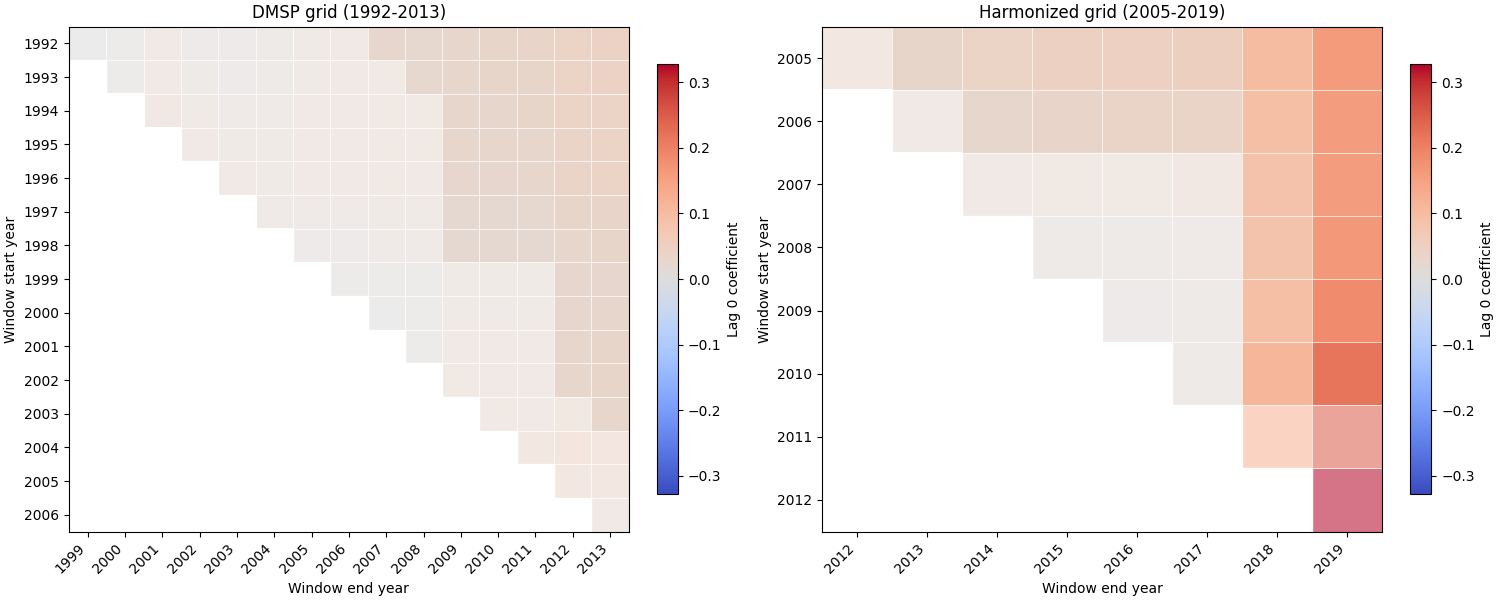
\includegraphics[width=\textwidth]{../analysis/Lag 0 birth-region coefficient across all valid windows.png}
\caption{Lag 0 birth-region coefficients across all valid start/end windows. The DMSP-only grid shows a broad block of positive coefficients, especially for mid-1990s starts and end years around 2007--2011, while the harmonized 2005--2019 grid remains close to zero throughout.}
\label{fig:first-stage-grid}
\end{figure}

\textbf{Interpretation of the nested-window and grid diagnostics.} The replication holds in the long DMSP-era sample and does not disappear immediately once the 1990s are excluded. The birth-region coefficient remains positive in 1995--2013 and remains positive, though weaker, in 2000--2013. The full DMSP grid sharpens that point: windows such as 1996--2010 and 1995--2010 produce coefficients around 0.02 with $p<0.001$, so the original first stage is not a knife-edge artifact of one endpoint choice. At the same time, the harmonized 2005--2019 grid does not recover a comparable signal. The full later window is essentially zero (0.0004, $p=0.966$), and even the strongest later window, 2012--2019, is imprecise (0.0136, $p=0.193$). Accordingly, the evidence is more consistent with a broad later-period weakening of the first stage than with a result driven exclusively by the late 1990s or by the fixed 2013 endpoint.

\textbf{Implications and remaining explanations.} These diagnostics reduce the plausibility of three simple explanations. First, the attenuation is not driven by the DMSP--VIIRS transition, because 2005--2013 remains entirely within the DMSP era. Second, it is not well summarized by a sharp decade break: the pooled $BirthRegion \times post2000$ and $BirthRegion \times post2010$ interactions are both statistically insignificant in the full 1992--2013 sample. Third, it is not rescued by alternative later start/end choices within the harmonized 2005--2019 sample, where the coefficients remain close to zero throughout the grid. Remaining possibilities include a smaller number of treated observations and clusters in the later window, weaker favoritism in the later political period, changes in country or leader composition, and attenuation specific to the post-2005 period rather than to a single decade indicator.

\subsection{Pollution-Side Results}
The pollution results follow directly from the replication diagnostics. Because the first-stage lights effect collapses in the later window, the environmental interpretation is constrained. The pollution regressions should therefore be read as evidence about later-period pollution dynamics in leaders' birth regions, not as a clean test of ``green favoritism'' built on a strongly replicated favoritism first stage.

Table~\ref{tab:main-results} reports the main pooled estimates in the ACAG sample. These coefficients do not support ``green favoritism.'' The nightlights effect is essentially zero, while the contemporaneous NO$_2$ effect is weakly positive and statistically significant at the 5 percent level. The pollution-intensity outcome, defined as log NO$_2$ minus log nightlights, is also positive and marginally significant. In substantive terms, the current pooled estimates suggest either no special growth effect in birth regions or slightly dirtier contemporaneous growth, not cleaner development. These pollution estimates cannot be interpreted in isolation. Because the nightlights first stage has itself collapsed in this period, the absence of green favoritism may simply reflect the absence of any detectable favoritism at all, rather than a finding about the environmental composition of directed growth.

\begin{table}[h]
\centering
\caption{Main pooled results (2005--2019)}
\label{tab:main-results}
\small
\begin{tabular}{lrrrr}
\toprule
Outcome & Coefficient & Std. Err. & p-value & N \\
\midrule
$\ln(\text{Nightlights}+0.01)$ & -0.0026 & 0.0091 & 0.778 & 631{,}377 \\
$\ln(\text{NO}_2+0.01)$ & 0.0308 & 0.0154 & 0.045 & 631{,}377 \\
Pollution intensity & 0.0333 & 0.0179 & 0.063 & 631{,}377 \\
\bottomrule
\end{tabular}
\end{table}

The heterogeneity checks ask whether the missing first stage reappears in the political settings where the theory would predict favoritism most strongly. So far that does not happen. The democracy interaction shows no meaningful birth-region effect in either nightlights or NO$_2$, and the interaction term itself is close to zero. Restricting the sample to stricter autocracies produces somewhat larger pollution-side coefficients, but not cleaner ones: in the $v2x\_polyarchy < 0.3$ subsample, the pollution-intensity coefficient is positive and statistically significant. That pattern leans away from the original ``green favoritism'' hypothesis and more toward a weak dirty-growth interpretation in the narrowest autocracy sample.

\begin{table}[h]
\centering
\caption{Heterogeneity checks}
\label{tab:heterogeneity}
\small
\resizebox{\textwidth}{!}{%
\begin{tabular}{llrrr}
\toprule
Specification & Outcome & Coefficient & Std. Err. & p-value \\
\midrule
Democracy interaction & $\ln(\text{Nightlights}+0.01)$: BirthRegion & -0.0032 & 0.0257 & 0.901 \\
Democracy interaction & $\ln(\text{NO}_2+0.01)$: BirthRegion & -0.0134 & 0.0406 & 0.741 \\
\midrule
Autocracy only ($<0.3$) & $\ln(\text{NO}_2+0.01)$ & 0.0682 & 0.0467 & 0.144 \\
Autocracy only ($<0.3$) & Pollution intensity & 0.1136 & 0.0530 & 0.032 \\
\bottomrule
\end{tabular}}
\end{table}

\begin{figure}[h]
\centering
\begin{minipage}{0.48\textwidth}
\centering
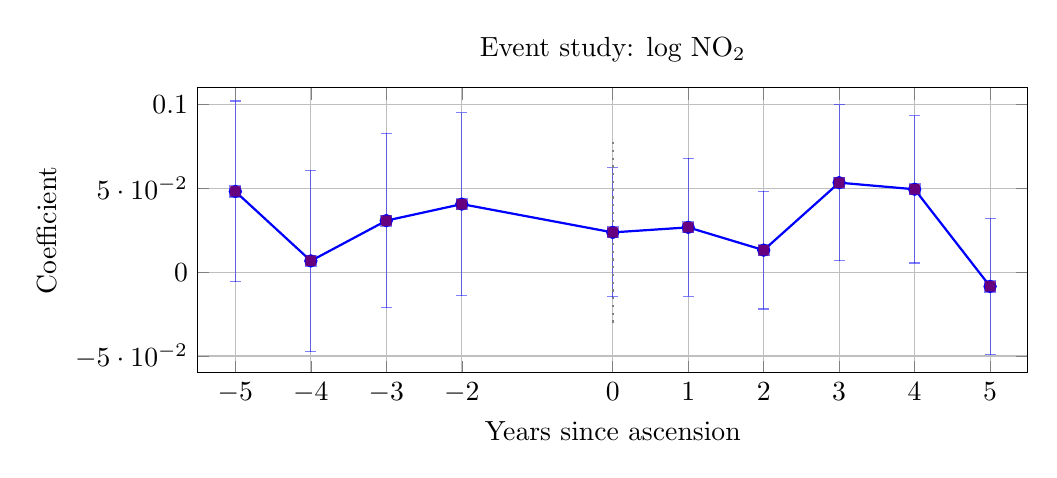
\begin{tikzpicture}
\begin{axis}[
    width=\textwidth,
    height=5.2cm,
    title={Event study: log NO$_2$},
    xlabel={Years since ascension},
    ylabel={Coefficient},
    xmin=-5.5, xmax=5.5,
    ymin=-0.06, ymax=0.11,
    xtick={-5,-4,-3,-2,0,1,2,3,4,5},
    grid=major,
]
\addplot[blue, thick, mark=*] coordinates {
(-5,0.04819) (-4,0.00676) (-3,0.03079) (-2,0.04065) (0,0.02376)
(1,0.02677) (2,0.01317) (3,0.05344) (4,0.04950) (5,-0.00847)};
\addplot+[blue, forget plot, opacity=0.5, error bars/.cd, y dir=both, y explicit]
coordinates {
(-5,0.048199) +- (0,0.053977)
(-4,0.006766) +- (0,0.054110)
(-3,0.030789) +- (0,0.052081)
(-2,0.040655) +- (0,0.054624)
(0,0.023763) +- (0,0.038462)
(1,0.026767) +- (0,0.041099)
(2,0.013175) +- (0,0.035115)
(3,0.053434) +- (0,0.046635)
(4,0.049501) +- (0,0.044013)
(5,-0.008467) +- (0,0.040784)};
\addplot[gray, dotted, thick] coordinates {(0,-0.03) (0,0.08)};
\end{axis}
\end{tikzpicture}
\end{minipage}
\hfill
\begin{minipage}{0.48\textwidth}
\centering
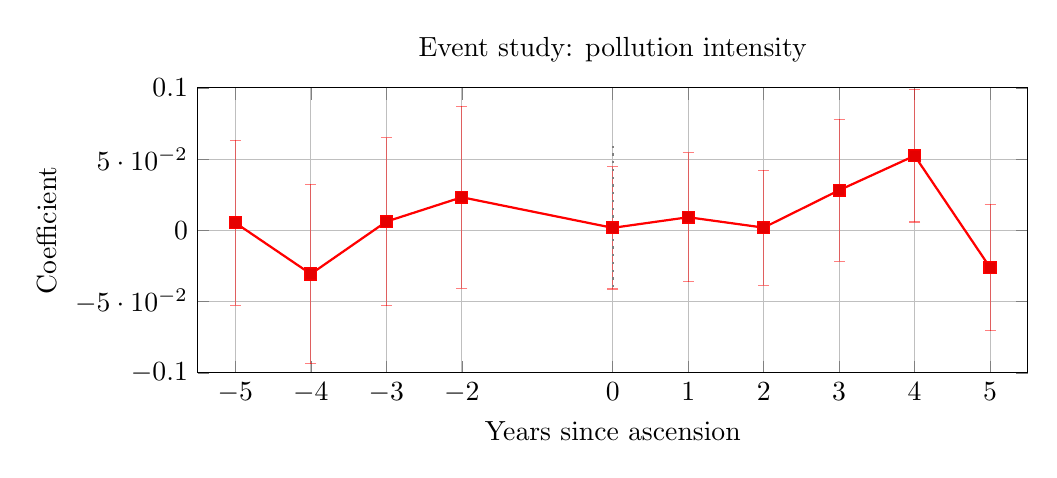
\begin{tikzpicture}
\begin{axis}[
    width=\textwidth,
    height=5.2cm,
    title={Event study: pollution intensity},
    xlabel={Years since ascension},
    ylabel={Coefficient},
    xmin=-5.5, xmax=5.5,
    ymin=-0.10, ymax=0.10,
    xtick={-5,-4,-3,-2,0,1,2,3,4,5},
    grid=major,
]
\addplot[red, thick, mark=square*] coordinates {
(-5,0.00527) (-4,-0.03065) (-3,0.00611) (-2,0.02323) (0,0.00175)
(1,0.00920) (2,0.00190) (3,0.02816) (4,0.05238) (5,-0.02614)};
\addplot+[red, forget plot, opacity=0.5, error bars/.cd, y dir=both, y explicit]
coordinates {
(-5,0.005285) +- (0,0.057993)
(-4,-0.030645) +- (0,0.063045)
(-3,0.006112) +- (0,0.058947)
(-2,0.023241) +- (0,0.063833)
(0,0.001750) +- (0,0.042919)
(1,0.009202) +- (0,0.045329)
(2,0.001901) +- (0,0.040388)
(3,0.028159) +- (0,0.049864)
(4,0.052383) +- (0,0.046566)
(5,-0.026134) +- (0,0.044358)};
\addplot[gray, dotted, thick] coordinates {(0,-0.04) (0,0.06)};
\end{axis}
\end{tikzpicture}
\end{minipage}
\caption{Event-study estimates with 95\% confidence intervals. The dynamics are not cleanly post-treatment: some pre-period movement remains, and the strongest positive coefficients appear only three to four years after ascension.}
\label{fig:event-study}
\end{figure}

The event studies point in the same direction, but they are not yet clean enough for a strong causal claim. The most notable positive NO$_2$ coefficients appear three to four years after leader ascension, and pollution intensity also turns positive around year four. However, there is already some movement in the pre-period, which means we cannot yet interpret the timing as clearly post-treatment.

A separate PM$_{2.5}$ analysis reinforces the broader pattern rather than overturning it. Table~\ref{tab:pm25} reports pooled estimates from the longer 1998--2024 sample. The treatment effect on log PM$_{2.5}$ is positive and statistically significant across all three lag structures, consistent with the NO$_2$ results above. Taken together, the pollution-side evidence is internally consistent: once the later-period first stage weakens, neither NO$_2$ nor PM$_{2.5}$ suggests that leaders channel cleaner growth to their birth regions.

\begin{table}[h]
\centering
\caption{PM$_{2.5}$ extension results (1998--2024)}
\label{tab:pm25}
\small
\begin{tabular}{lrrrr}
\toprule
Lag & Coefficient & Std. Err. & p-value & N \\
\midrule
Lag 0 & 0.0063 & 0.0027 & 0.018 & 1{,}289{,}925 \\
Lag 1 & 0.0060 & 0.0027 & 0.025 & 1{,}289{,}925 \\
Lag 2 & 0.0058 & 0.0027 & 0.031 & 1{,}289{,}925 \\
\addlinespace
Outcome & \multicolumn{4}{l}{$\ln(\text{PM}_{2.5}+0.01)$} \\
Region FE & \multicolumn{4}{l}{Yes} \\
Country-year FE & \multicolumn{4}{l}{Yes} \\
\bottomrule
\end{tabular}
\end{table}

\section{Plan for Remaining Work}
\noindent The data infrastructure is now in place. The central challenge for the final report is interpretive: the classic favoritism first stage is strong in the long historical sample but weak in the 2005--2019 window where pollution data exist. The remaining work addresses this in three stages.

\begin{enumerate}[leftmargin=*]
    \item \textbf{Resolve the first-stage attenuation.} Determine whether the nightlights effect survives in strict-autocracy subsamples ($v2x\_polyarchy < 0.3$), in the DMSP-only 2005--2013 window, or in specific country groups. This will determine whether the final paper can condition the pollution analysis on a credible first stage or must instead frame the attenuation itself as the main finding.
    \item \textbf{Strengthen the pollution-side evidence.} Test sensitivity to alternative outcome transformations and formally compare NO$_2$ and PM$_{2.5}$ results to assess whether they tell a consistent story.
    \item \textbf{Settle the paper framing.} Based on the results of steps 1 and 2, commit to one of two narratives: (a)~a heterogeneity paper showing that favoritism and its environmental footprint persist in autocracies, or (b)~a later-period null-result paper documenting the attenuation of classic favoritism and the absence of green favoritism in the pollution era.
\end{enumerate}

\section{Updated Responsibilities}

\begin{itemize}[leftmargin=*]
    \item \textbf{Richard Schulz} will run additional pollution robustness checks (alternative log transformations), produce publication-style regression tables, and draft the final paper narrative including the framing decision between an attenuation story and a heterogeneity story.
    \item \textbf{Muhammad Majid Altaf} will extend the PM$_{2.5}$ analysis with event-study and heterogeneity specifications, assess whether PM$_{2.5}$ offers a stronger or more interpretable pollution signal than NO$_2$, and prepare the PM$_{2.5}$ results for inclusion in the final report.
    \item \textbf{Ruby Wang} will investigate the first-stage attenuation by testing whether the nightlights effect survives in strict-autocracy subsamples and in the DMSP-only 2005--2013 window, and will run diagnostics on changes in country and leader composition across sample periods.
\end{itemize}

\section{Questions for Feedback}
\begin{enumerate}[leftmargin=*]
    \item The nightlights first stage is strong in the long 1992--2013 sample but essentially zero in the 2005--2019 window where our pollution data exist. Should the final paper focus on (a)~documenting this attenuation as the main result, or (b)~restricting to subsamples where the first stage survives (e.g., strict autocracies) and framing the paper around heterogeneity in favoritism and pollution?
    \item We can invest remaining time in several directions: adding more pollution robustness checks (alternative transformations, additional pollutants), improving the event-study design (confidence intervals, sharper pre-trend tests), or narrowing the sample to strengthen the first stage. Which of these would be most valuable for the final report?
\end{enumerate}

\end{document}
